\subsubsection{Exercise} 


Figure \ref{min_dyn_fig} shows the reaction of the minimum phase system.

Figure \ref{nonmin_dyn_fig} shows the reaction of the non-minimum phase system.

See Table \ref{analysis_dyn} for the analysis of the results. 

\begin{figure}[h!t]
        \centering
        \begin{subfigure}[b]{\columnwidth}
                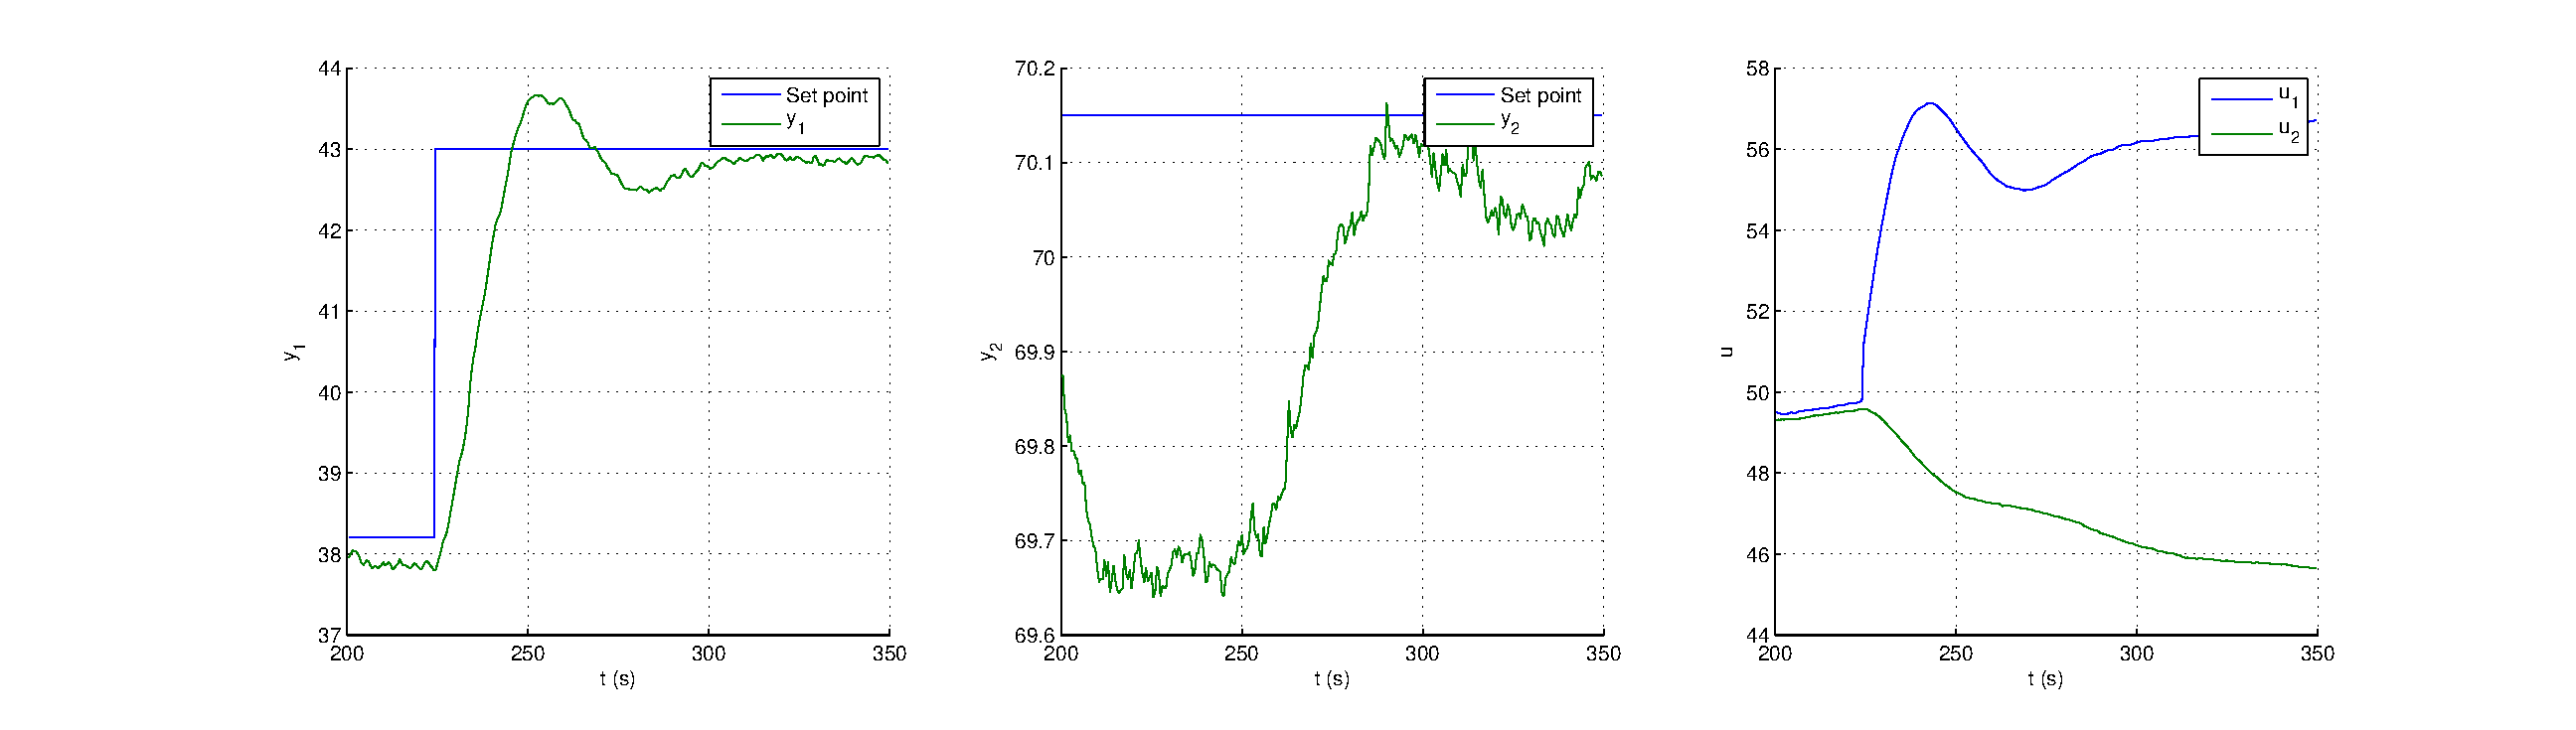
\includegraphics[width=\columnwidth]{fig/min_dyn_step.eps}
                \caption{Step response}
        \end{subfigure}
        \begin{subfigure}[b]{\columnwidth}
                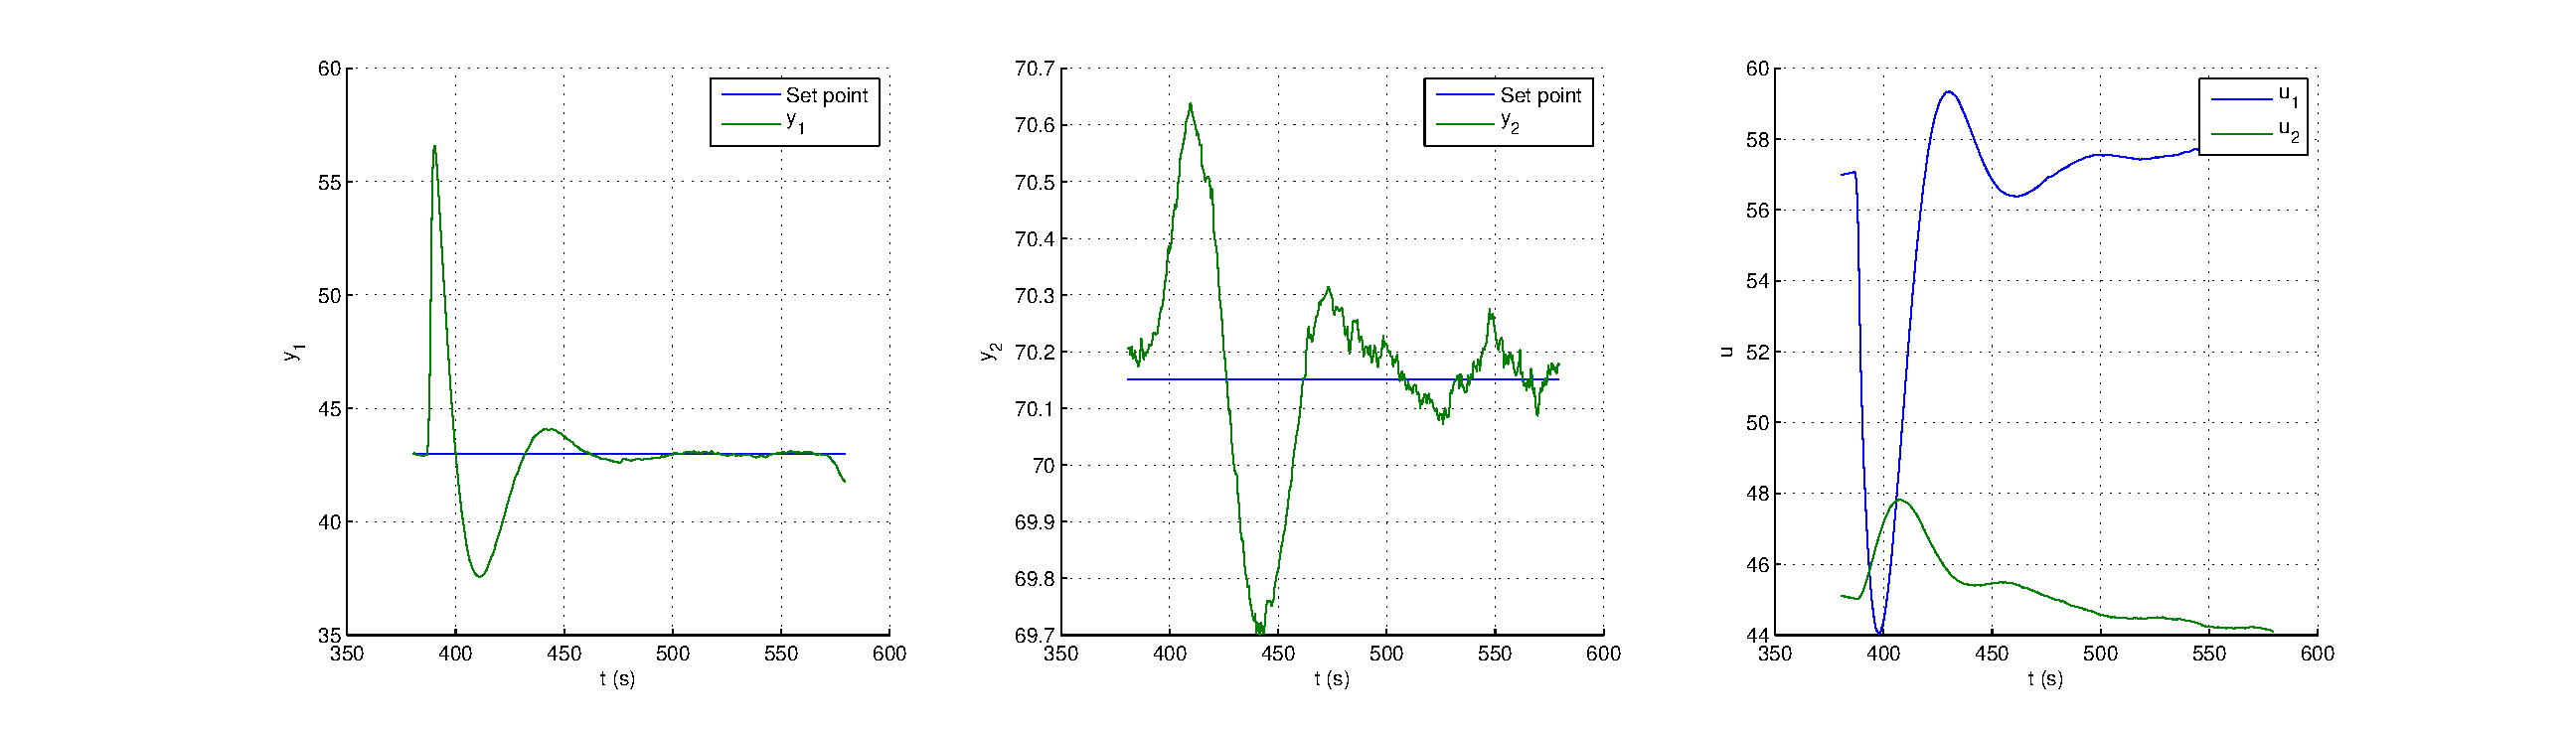
\includegraphics[width=\columnwidth]{fig/min_dyn_gob.eps}
                \caption{Cup of water response}
        \end{subfigure}
        \begin{subfigure}[b]{\columnwidth}
                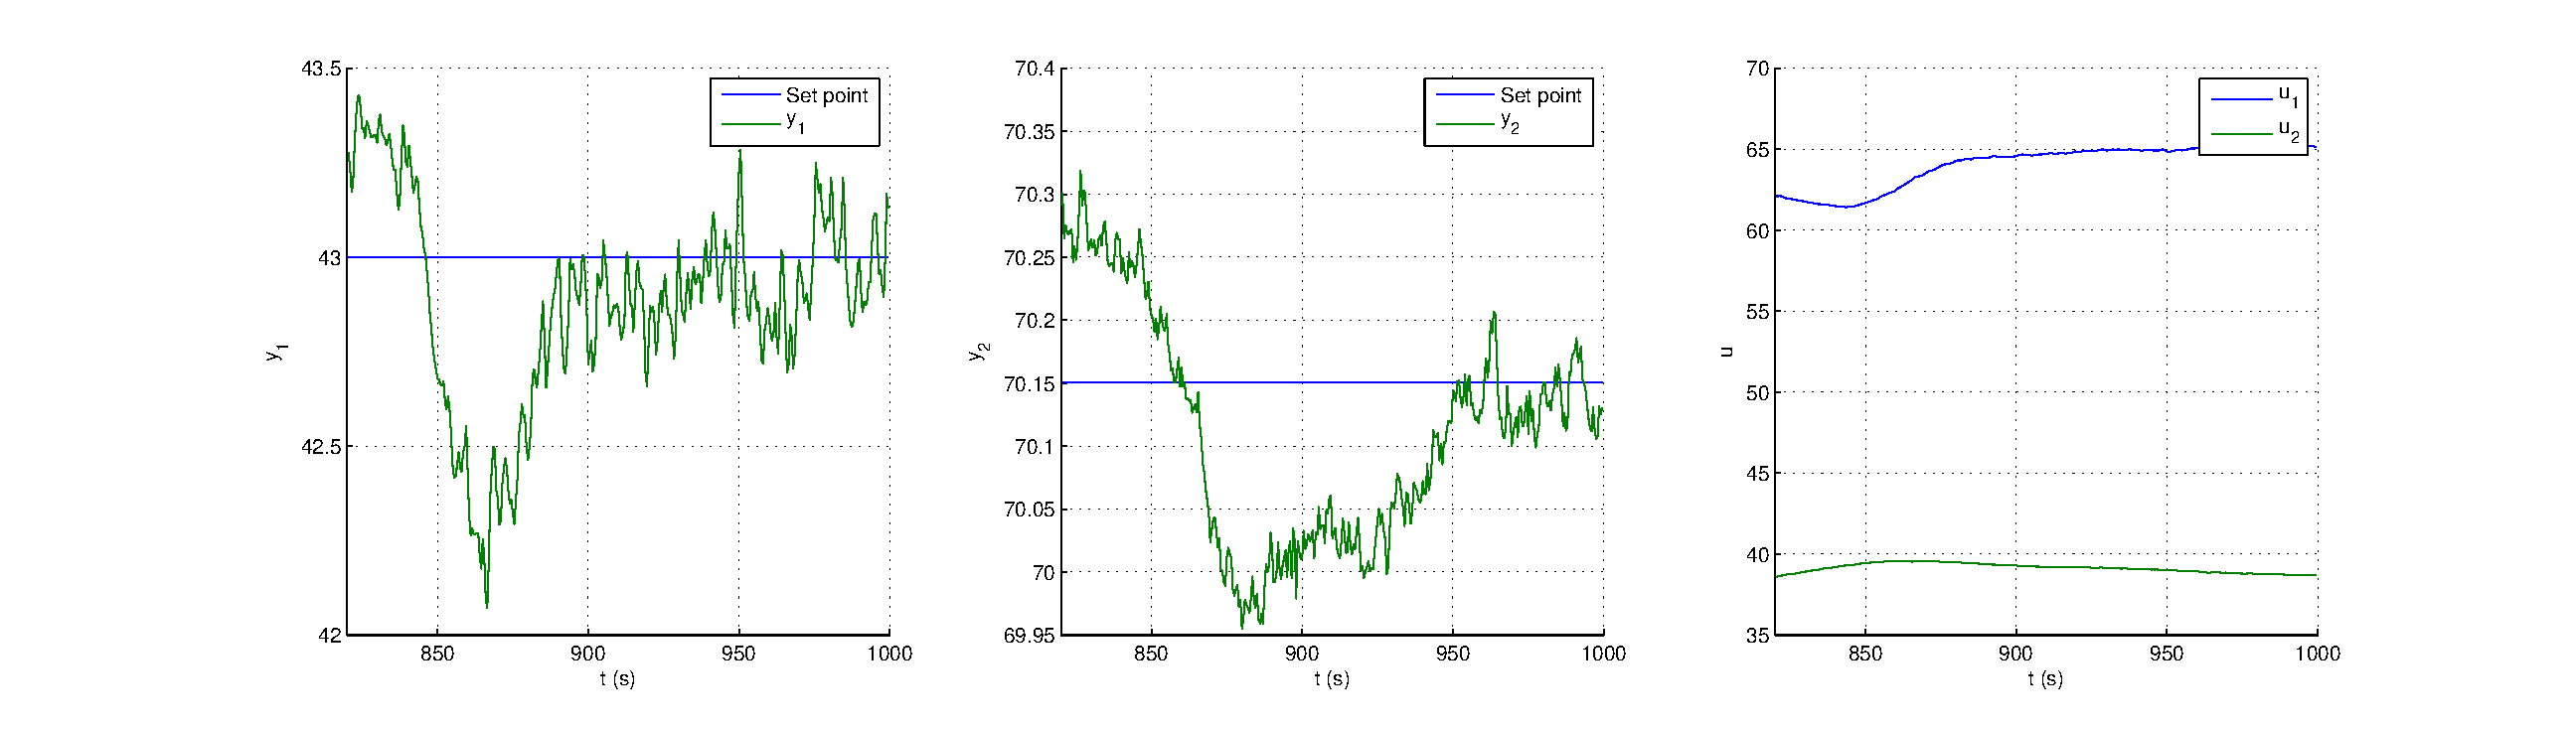
\includegraphics[width=\columnwidth]{fig/min_dyn_fui.eps}
                \caption{Extra outlet response}
        \end{subfigure}
        \caption{Minimum phase system reactions \\ Decentralized controller}
        \label{min_dyn_fig}
\end{figure}

\begin{figure}[h!t]
        \centering
        \begin{subfigure}[b]{\columnwidth}
                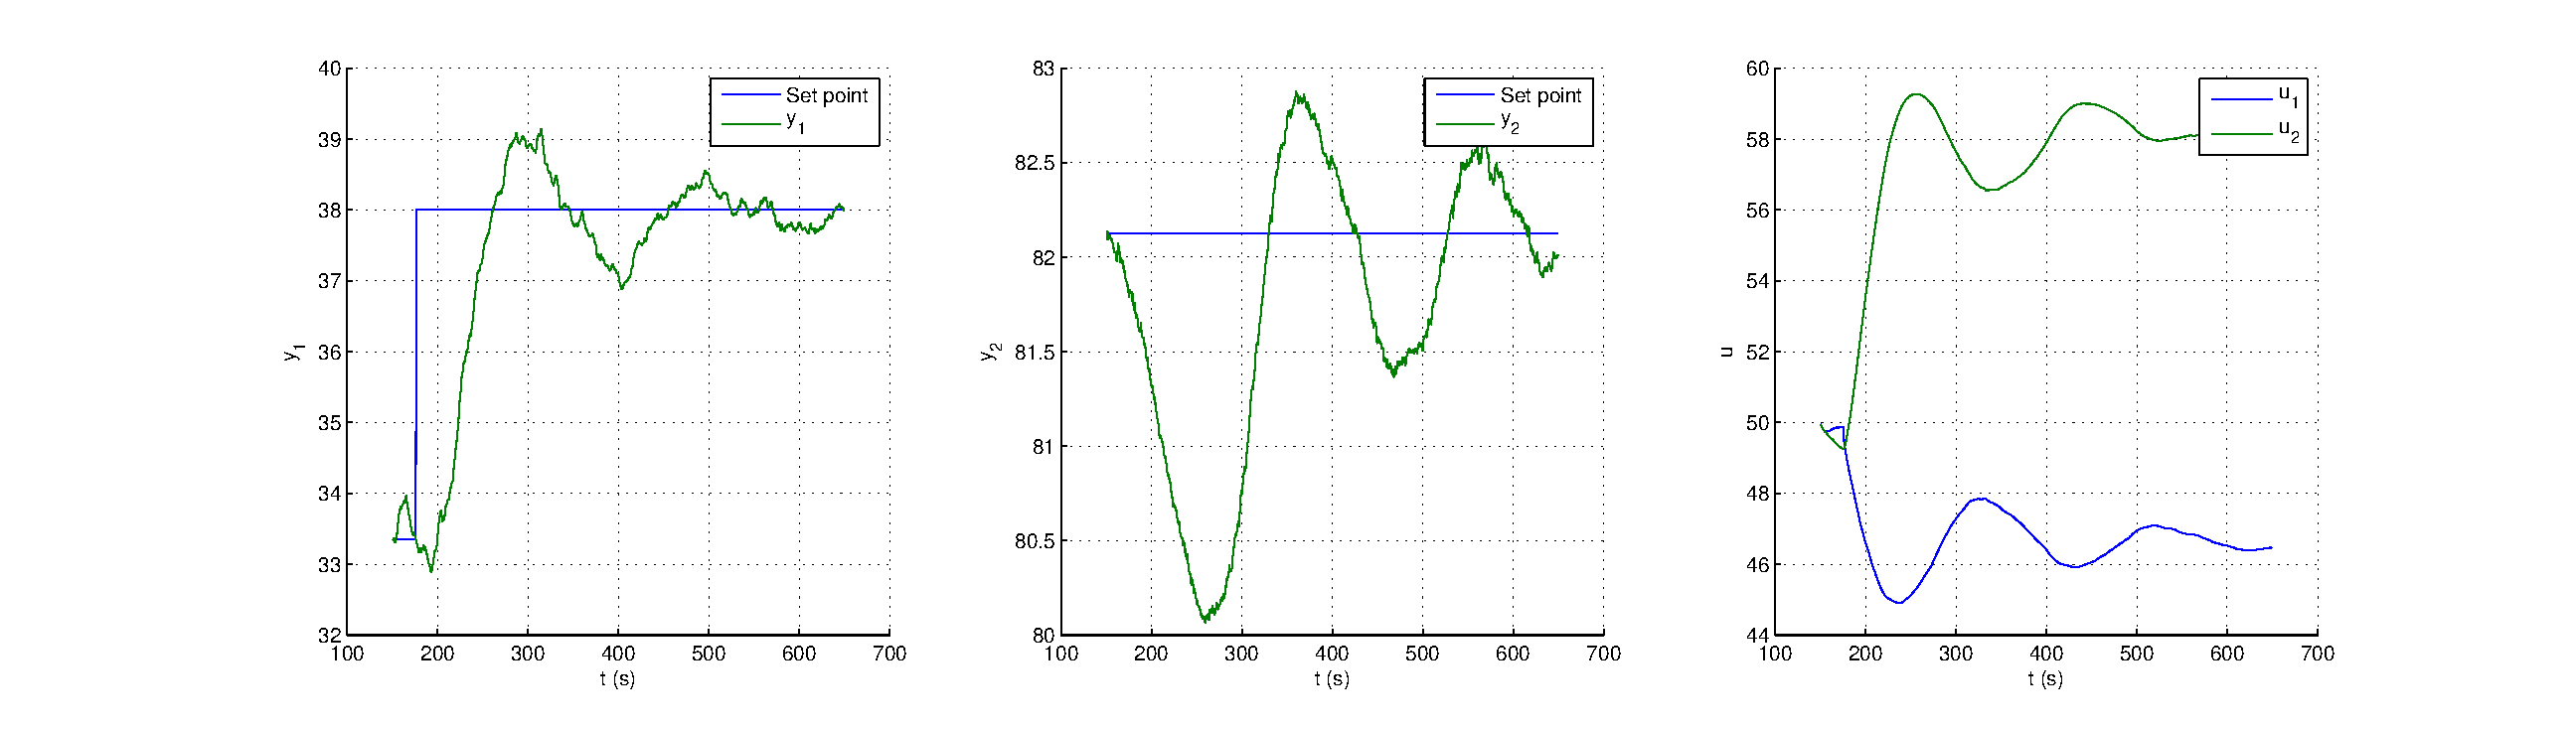
\includegraphics[width=\columnwidth]{fig/nonmin_dyn_step.eps}
                \caption{Step response}
        \end{subfigure}
        \begin{subfigure}[b]{\columnwidth}
                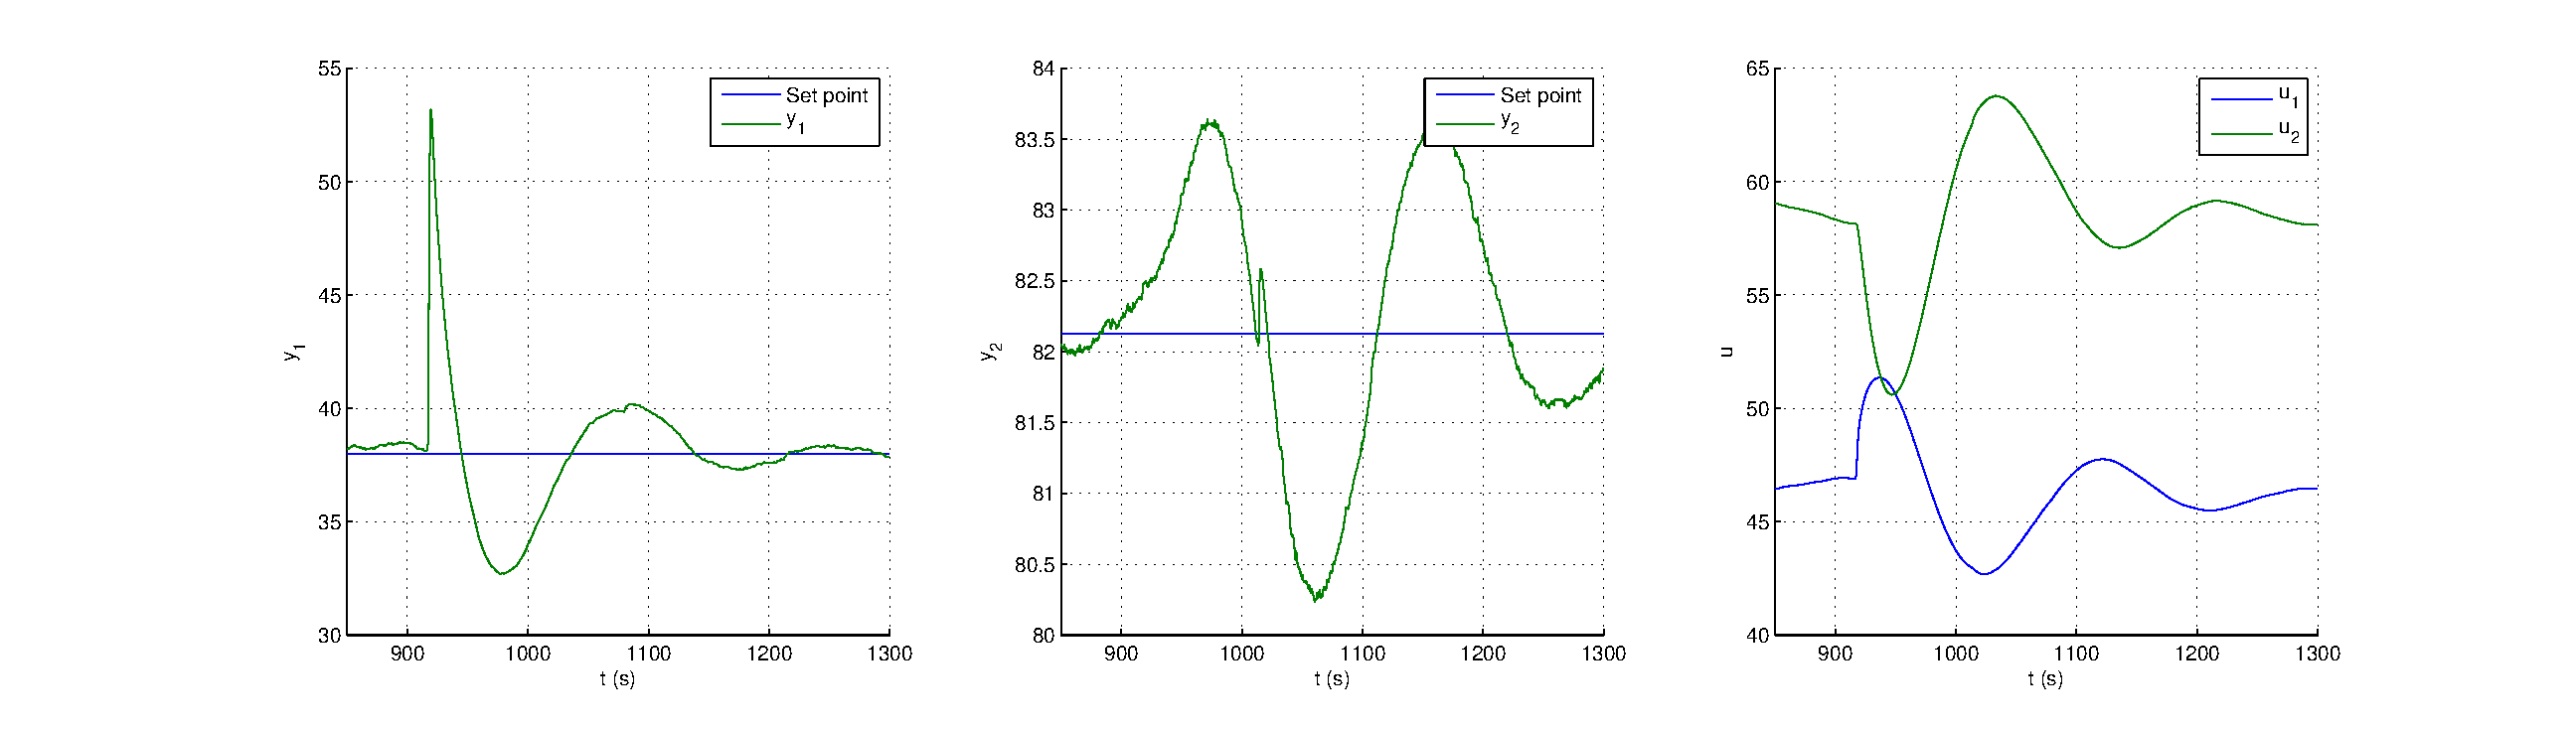
\includegraphics[width=\columnwidth]{fig/nonmin_dyn_gob.eps}
                \caption{Cup of water response}
        \end{subfigure}
        \begin{subfigure}[b]{\columnwidth}
                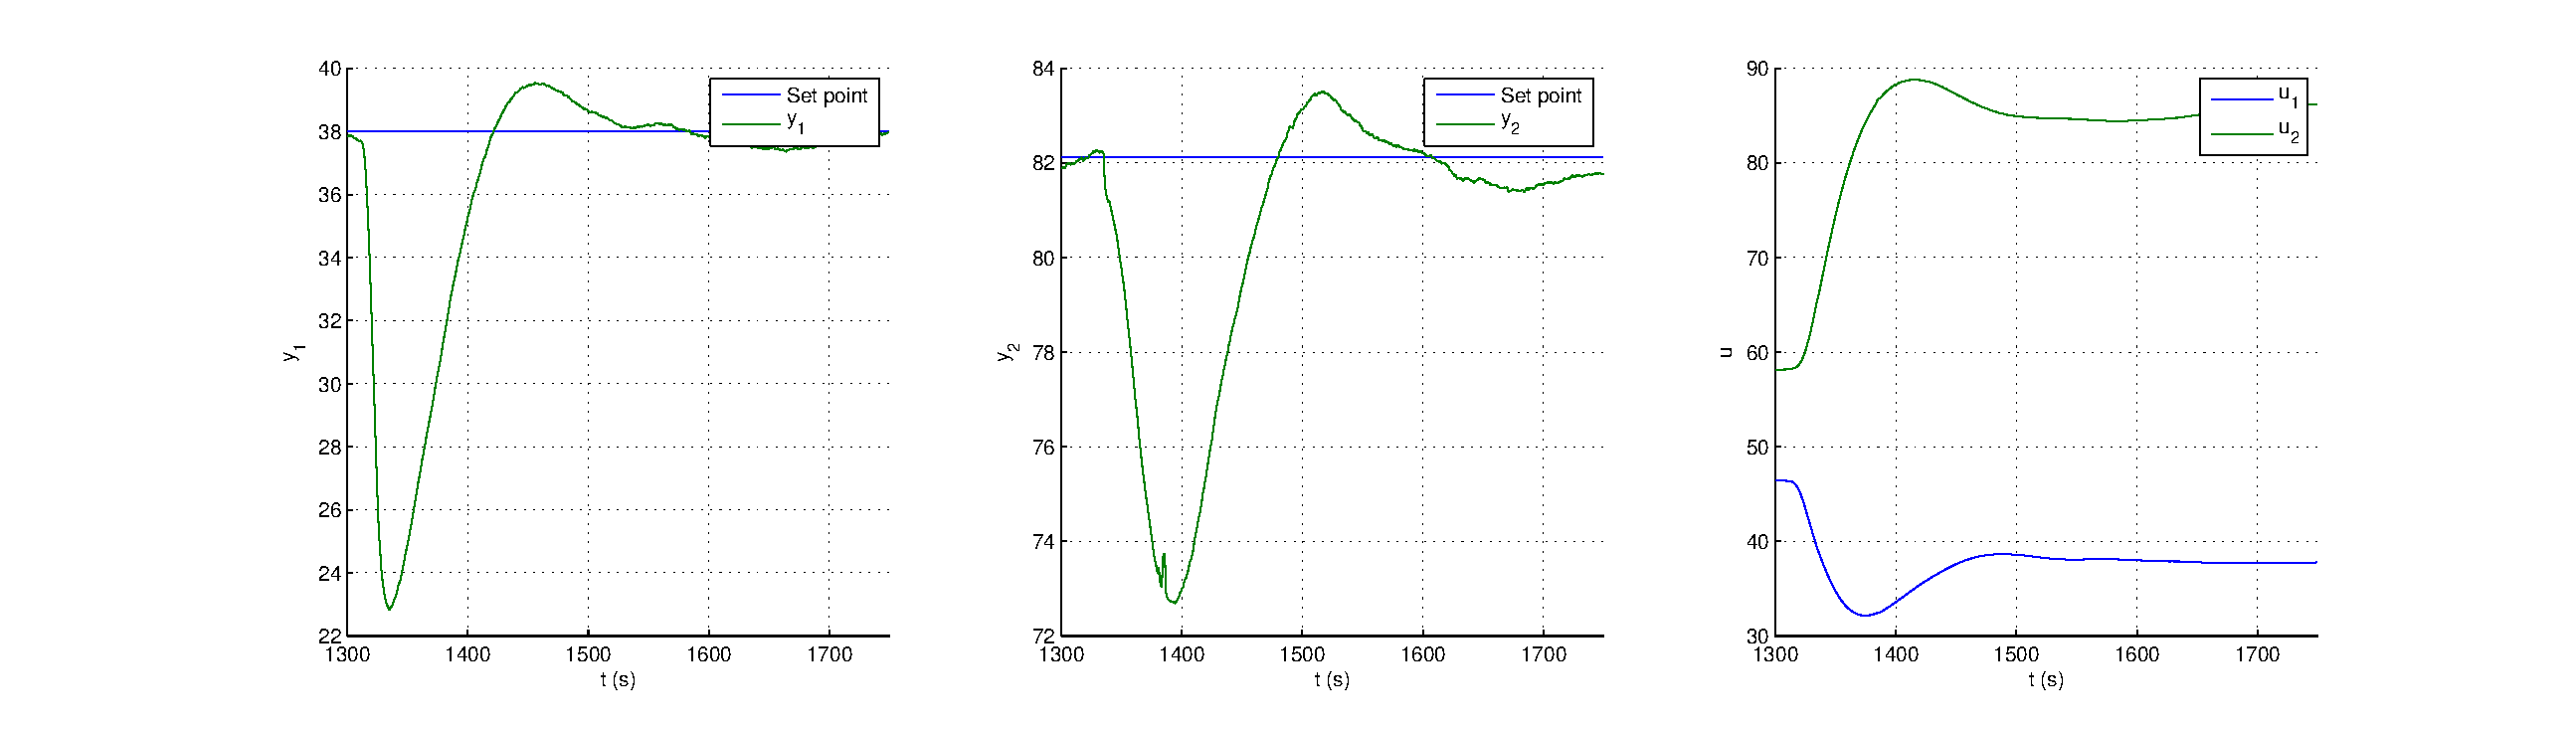
\includegraphics[width=\columnwidth]{fig/nonmin_dyn_fui.eps}
                \caption{Extra outlet response}
        \end{subfigure}
        \caption{Non-minimum phase system reactions \\ Decentralized controller}
        \label{nonmin_dyn_fig}
\end{figure}

\begin{table}[h!t]
    \centering
    \begin{tabular}{|c|ccc|}
        \hline
        & Rise & \multirow{2}*{Overshoot} & Disturbance \\
        & time & & rejection \\
        Minimum phase & & & \\
        Non-minimum phase & & & \\
        \hline
    \end{tabular}
    \caption{Step response and load disturbance analysis \\ Decentralized controllers}
    \label{analysis_dyn}
\end{table}
